\begin{savequote}[8cm]
\textlatin{Neque porro quisquam est qui dolorem ipsum quia dolor sit amet, consectetur, adipisci velit...}

There is no one who loves pain itself, who seeks after it and wants to have it, simply because it is pain...
  \qauthor{--- Cicero's \textit{de Finibus Bonorum et Malorum}}
\end{savequote}

\chapter{\label{ch:35-nuint}Neutrino interactions} 


\section{TKI}
\label{sec:nuint-tki}
\minitoc

\begin{figure}[!htb] 	
    \centering 		
    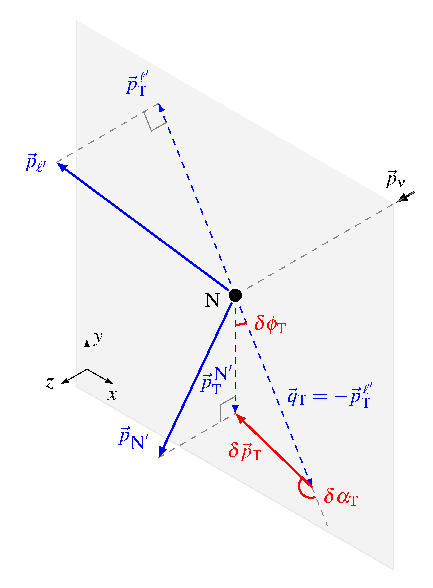
\includegraphics[width=0.35\textwidth]{figures/stki.eps}
    \caption{\label{fig:stki} Schematic illustration of the TKI variables. Diagram taken from Ref.~\cite{Lu:2015tcr}.} 
\end{figure}

The TKI variables are shown in Fig.~\ref{fig:stki}. They are cleverly constructed such that they are most sensitive to IS and FSI. 
In the simplest case, there are only two final particles after the neutrino-nucleon interaction, a muon and a proton. 
If the initial momentum of the struck nucleon has no component transverse to the neutrino's incoming direction, the products, i.e. the muon and the proton, should not have a net transverse component either, unless the struck nucleon has a non-zero initial transverse component or the final particles have undergone FSI.
Suppose there is no FSI, the net transverse component, $\dpt$, corresponds exactly to the magnitude of the transverse component of the struck nucleon, and the angle, $\dat$, represents the direction of the initial nucleon motion projected on the transverse plane. 
Assuming the nucleons are moving isotropically, the $\dat$ distribution should be flat. 
All current nuclear models do not have a preferential direction for initial nuclear motion, so it is only natural to assume the nucleons move in random directions. 
Thus, the deviation from flatness for $\dat$ can only be due to FSI, thereby making it an excellent probe for FSI. 
As for $\dpt$, it reflects the magnitude of the initial nucleon momentum transverse to the neutrino direction compounded by FSI. 
Furthermore, if the nucleus is assumed to be at rest and no other particles are knocked out other than the muon and the proton, the initial nucleon momentum, $\pn$, can also be derived following the steps outlined in \cite{pnpaper}. 
 